% Proposal for the features and scoring and stuff of my senior project.
\documentclass{article}
\title{Senior Project Presentation}
\author{Steve Jarvis}
\date{\today}
% Disables chapter and section numbering
\setcounter{secnumdepth}{-1} 
\usepackage[pdftex]{graphicx}
\usepackage{listings}

\begin{document}
\maketitle

\section{What I Learned...}
\subsection{What's a Neural Network?}
    \paragraph{}A neural network is a general machine learning tool that can be used to 
    learn a large variety of data sets. A neural network is a set of connected weights,
    and the nodes of the network are activations of the input based on the corresponding
    weights.
    \paragraph{}The simplest neural network is one consisting of two layers. A weight
    connects each node in the first layer to each node in the second layer. For example,
    the following diagram could represent a two-layer network used to learn the OR logic
    gate. Imagine three input nodes and two output, with the bottom left representing false
    and the bottom right true. When inputting bits representing logical OR, the network
    should yield output representing true. See Figure~\ref{basicnetwork} on 
    page~\pageref{basicnetwork} for an illustration.
    \paragraph{}An important consideration for this sample network is its limited learning
    ability. A two-layer network can only learn linearly separable functions; equations
    whose positive and negative results, when graphed, could be partitioned by a single line.
    More complex functions require deeper networks to learn, although the complexity
    increases quickly. With only a single extra layer (and ~200 nodes per layer) the
    neural net was able to achieve 93 percent accuracy on the MNIST Database of Handwritten
    Digits\footnote{http://yann.lecun.com/exdb/mnist/}.
    \begin{figure}
        \centering
        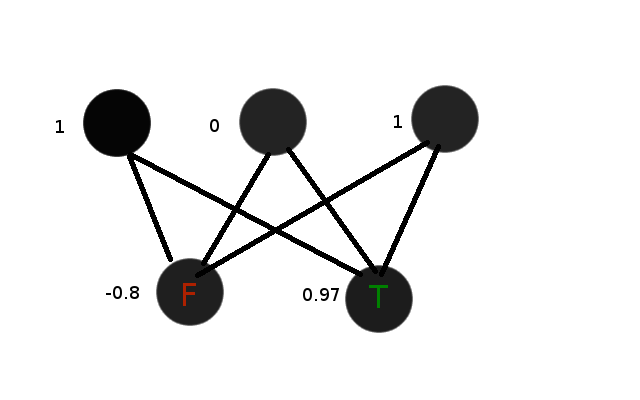
\includegraphics[scale=0.4]{images/perceptron.png}
        \caption{The top layer are inputs, connected by weights to the bottom layer. The
            weights are changed during training so that they give the desired output for
            the right input. A common implementation is to use functions with a range such 
            that -1 < y < 1, so assuming the network is trained to represent true with 1 
            and false with -1, this would be a great output.}
        \label{basicnetwork}
    \end{figure}
\subsection{Why Is There An Extra Input Node?}
    \paragraph{}The third input node is called a bias. The purpose of a bias is to allow
    any necessary shifting of the activation function. For example, the activation function
    for the network used in this project is the hyperbolic tangent. It was used because the
    domain is all real numbers, it is smooth, continuous, and symmetrical, and the range
    is -1 to 1. It is also easily derived, which is becomes important later in training. As
    the weights change, the steepness of the graph is changed, but the y-intersect is always
    0. The bias node allows the shifting of the entire graph, which is the only way to train
    something other than a 0 output for a 0 input.
    \begin{figure}
        \centering
        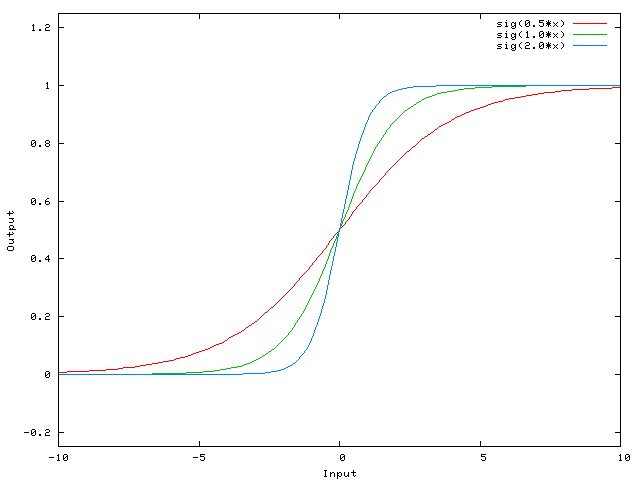
\includegraphics[scale=0.4]{images/bias.png}
        \caption{The graph of a general sigmoidal function as the coefficients (weights)
            change. Pic taken from StackOverflow: http://stackoverflow.com/questions/2480650/role-of-bias-in-neural-networks}
    \end{figure}
\subsection{How Are the Correct Weights Calculated?}
    \paragraph{}Finding the right weights is all the work. The correct weights are found
    via a process called back propagation. Back propagation is a repeated process of error 
    correction, starting with the output nodes and moving back up the network. The error
    of the output nodes is simply the difference between the desired output and the actual
    output, but the error calculation for each node higher up the tree must be a function
    of the collective error of the exiting connections, since each node is connected to each
    node in the level down. This algorithm proved to be the most difficult part of the project
    and I consulted numerous and tutorials and open source projects online.\footnote{Here are
    some of the most helpful resources I found: \\  
    http://www.cs.montana.edu/~grayd/backprop.htm \\ 
    http://arctrix.com/nas/python/bpnn.py}
    \paragraph{}The network is always training in the background so the user can see 
    potentially constant improvement, and to learn more and different handwriting there 
    only needs to be more data added to the instance on the server. Also, the network takes 
    very long to train. At the time of this presentation, this network will have been 
    training on euclid for about a month, and that's not unusual. Because of the dependency on 
    adjacent layers in back propagated training, it can not be efficiently parallelized\footnote{https://research.microsoft.com/apps/pubs/default.aspx?id=173312}.
    \paragraph{}Earlier it was mentioned that hyperbolic tangent is easily derived and that's
    nice for training. That is because we can use the derivative of the activation function
    in calculating the weight deltas. Consider how the derivative changes as the function
    is traveled. Since the derivative is greatest at the middle -- where the activation is
    most uncertain -- results in the middle will cause a greater change in the associated
    weights. Conversely, as the network's weights become more established through training, 
    the derivative approaches zero and the network stabilizes.
\subsection{iOS, JSON, and CGI.}
    \paragraph{}I wanted a good way to demonstrate the neural network. Just knowing it could
    recognize handwritten characters from a database is not very exciting, but having it 
    recognize a user's in real time would be. So an iOS front end was added to take input, 
    query the server on which the network is running, and return an ordering of likeliness, 
    from 0 to 9, of which digit it was sent. The only particular I'd like to mention is how
    surprisingly easy it was get Apache to interpret Python files. This file in a pub
    directory on euclid is all it takes. \\

    \begin{lstlisting}
    file .htaccess

    euclid is down I cannot remember what I wrote...
    \end{lstlisting}

\section{Software Organization...}
    \paragraph{}I chose to have an independent neural network, and I still like that 
    decision. What could use improvement is the way it is incorporated with the rest of 
    the project. There are multiple applications that rely on the neural network module

\section{Complex Data Structures and Algorithms...}
    Machine learning is hard

\section{As Hard As I Expected...}
    \paragraph{}I was expecting really hard, and it's about what I got. I have an anecdote to
    demonstrate. When I first starting trying to train handwritten digit recognition I didn't
    get any performance better than ~15\%. I would let the network train for days on even small
    samples of data, and it would just top out. Worse still, it was unpredictable. This is
    why I added the "experiment" mode to the network training application. I could see that 
    "skinny" three-layer networks -- networks with fewer than about 60 nodes per layer -- mastered
    data sets quickly and flawlessly. As the networks grew larger they became wildly inconsistent.
    So the experiment trained a constant function with a constant number of iterations to
    increasingly large networks and graphed the error rate and time to complete versus size.
    Figure~\ref{badgraph} shows the inital results. This was completely bewildering to me for about
    a week, especially since I tried tweaking the learning coefficients. There are just so many
    moving pieces that I couldn't imagine what the issue might was. It turns out the answer was
    local minima, and that turning the learning and momentum rates way down would help to avoid
    getting stuck in them. Figure~\ref{goodgraph} shows the nearly flawless performance of
    the improved network.
    \paragraph{}The next great challenge was improving the disappointingly poor performance of
    real life digit recognition. The network was training on euclid as I was finishing the basic
    functionality of the iOS application, and by the time I finished the logs read it was
    correctly recognizing more than 93\% of the test data. In actual use, however, I found the
    network to correctly interpret only the nicest of input. The problem was the strict 
    preprocessing done to the data in the MNIST Database did not represent data thrown in from
    the real world. To improve real life performance, I "messied" up the data by changing the
    size and rotation. The variations I added turned the training set of ~40k samples into a
    set of ~1.5M samples. 
    \paragraph{}After swapping the training data, the learning curve became stagnant
    at about 70\% success. The messier data set was too complex for a three-layer network to learn,
    so I added a fourth layer. Similar to the bump from two to three, the change from three to
    four meant lower learning rates to avoid the increased chance of becoming stuck in local
    optima and longer training times to facilitate the exponentially increasing number of
    connections. Alas, it seems to be working with acceptable performance. To further increase
    the performance, I believe finding an appropriate bounding box per submitted sample on
    the iOS application would yield noticable improvements.

    \begin{figure}
        \centering
        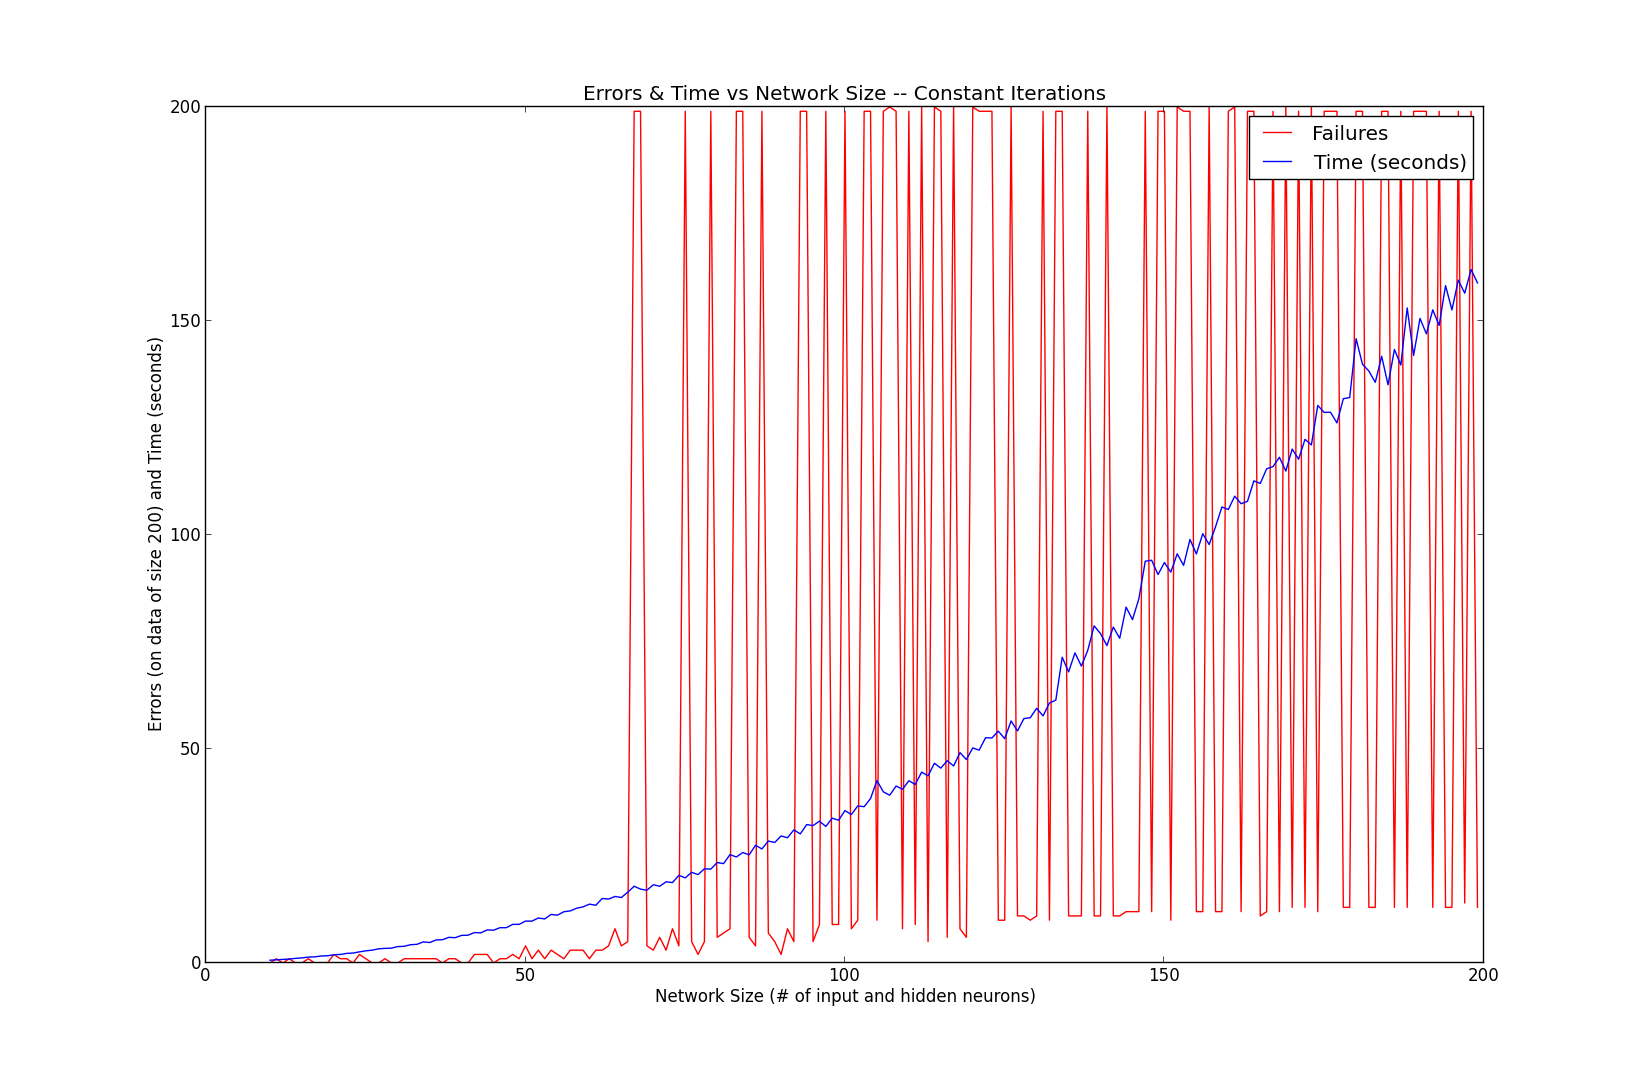
\includegraphics[scale=0.4]{images/bad_learning.png}
        \caption{The experiment run with the initial learning rate}
        \label{badgraph}
    \end{figure}

    \begin{figure}
        \centering
        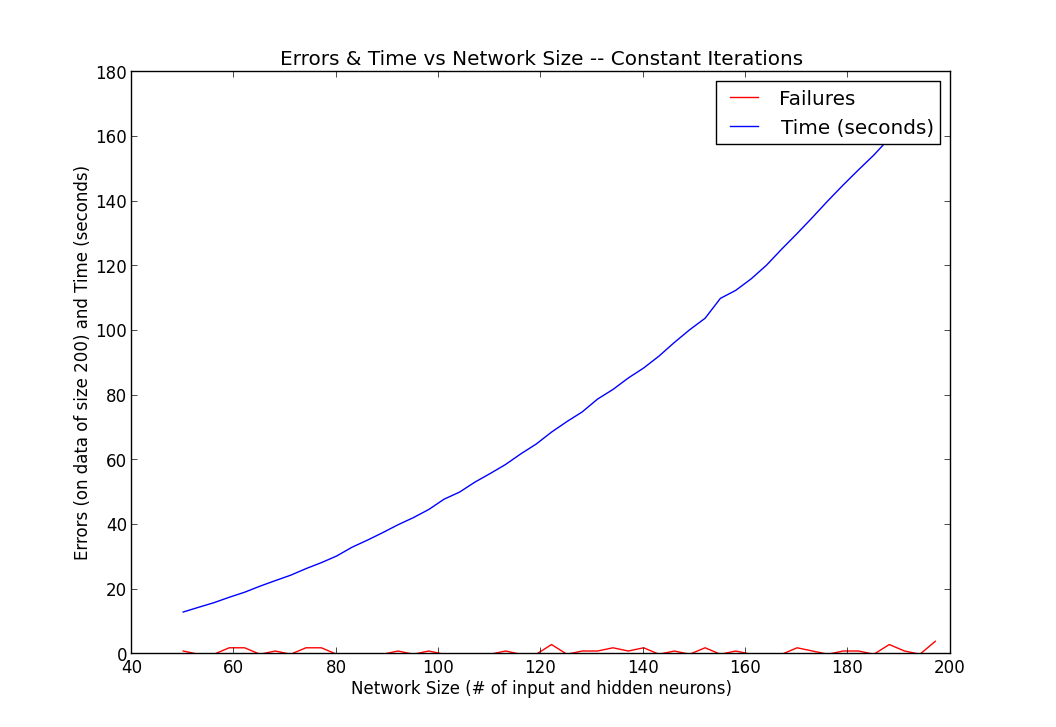
\includegraphics[scale=0.5]{images/good_learning.png}
        \caption{The experiment run with a learning rate and momentum rate 1/1000th of
            the initial size}
        \label{goodgraph}
    \end{figure}

    \paragraph{}Here are the approximate line 
    counts\footnote{iOS App is Modified GLPaint from Apple: https://developer.apple.com/library/ios/\#samplecode/GLPaint/}. \\

    \begin{tabular}{ l c r }
        Part & Line Count & Language \\
        \hline \\
        Neural Network & 542 & Python \\
        Network Training & 1142 & Python \\
        Web Site & 67 & Python \\
        iOS App & 1564 & Objective C \\
        Total & 3315 & All \\
    \end{tabular}

\end{document}
